\chapter{Introduction}
Within the recent years, we have seen an incredible growth in the gaming industry. Newzoo, a leading provider of games market intelligent, reported that “the gaming industry is growing faster than expected, up 10.7\% to \$116 billion 2017” \cite{_newzoo:_????}. As visible in Figure \ref{fig:newzoo2}, half of the global game market is represented by the mobile industry, including tablets and smartphones and the future perspectives show a continuous growth at an annual rate of 8.2\% up to 2020. 
\begin{figure}
    \centering
    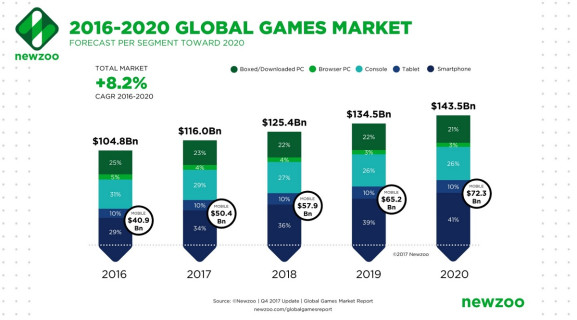
\includegraphics{masters-thesis-master/masters-thesis/contents/01_introduction/newzoo-2.jpg}
    \caption{Trend of the mobile game industry from 2016 to 2020. Image from \cite{_newzoo:_????} }
    \label{fig:newzoo2}
\end{figure}
Furthermore, as showed in Figure \ref{fig:newzoo3} the mobile market segment is growing faster compared to the other segments in the game industry, with a year on year growth rate of 23.3\% in 2017.
\begin{figure}
    \centering
    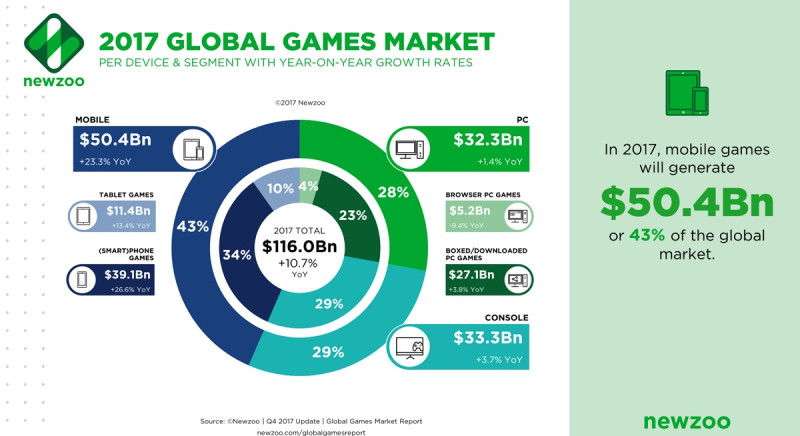
\includegraphics[width=\textwidth]{masters-thesis-master/masters-thesis/contents/01_introduction/newzoo-3.jpg}
    \caption{Per device and segment global games market and year-to-year growth rates . Image from \cite{_newzoo:_????} }
    \label{fig:newzoo3}
\end{figure}
Everyday more and more people use their tablet or smartphone to play video games and a recent report on Verto Analytics \cite{_report:_2016} showed that gamers play an average of 24 minutes each day. These incredible numbers motivate why it is important to deeper understand what is going on in this sector and which implications are emerging. First of all, a key factor in this growth is the cheaper and higher quality technology as well as the possibility of accessing Internet almost everywhere, enabling the development of more engaging games. As an example, nowadays is easy to play a game online, together with a friend, sharing achievements, competing in a leader-board or exchanging virtual gifts. But just like the technologies and the way we play video games has changed, also the way game companies make money from video games has changed too. 

\section{From Pay-to-Play to Free-to-Play Business Model}
A current trend is the shift from the traditional Pay-to-Play (P2P) business model to the Free-to-Play (F2P) or “freemium” business model. The F2P model allows users to acquire and play a game free of charge and at the same time, encourages them to pay for in game additional content  with different purpose, e.g. unlocking content, avoiding ads, buying boosters, etc. More than that, it allows game companies to increase the popularity of a game and to collect revenues later on. On the contrary, the P2P business model describes those game where the user must pay before obtaining the game and then the game content is free. Previously, the players paid once and then they played as mush as they wanted. Now,  the potential profit of a single game is theoretically infinite dollars. This shift is demonstrated by the tremendous success of many F2P games like Candy Crush Saga (King.com 2012), Clash Royal (Supercell 2016) or Hearthstone (Blizzard Entertainment 2014). Even if there are also some example of profitable P2P games like Minecraft (Microsoft Studios 2011), the evidence of this shift is indicated by the fact that Apple Store is dominated by apps that use a F2P business model. The free-to-play business model dates back to  1999 when it was first used in the Nexon's QuizQuiz game, made by Lee Seungchan. However is only in the last decade that it has become the leading way of monetizing games.

To be precise, also slightly different business models are possible. World of Warcraft (WoW), a multiplayer online game (Blizzard Entertainment 2004), is an example of a game where the user needs to pay to maintain an active account. However, since the player has no choice and he must pay if wants to play the game, we will consider it as a P2P game. Finally, demos can be considered as F2P games since the player can try the game for free and decides later if buying or not the game. 

A key factor in favour of the F2P business model is the low or almost zero barriers for new users, since the game requires only a smartphone and a good enough internet connection to be downloaded. This allows F2P games to acquire large scale visibility and a bigger user base. Another important aspect that has favored this shift is the change in the market user base. Nowadays, gaming is a mass market and most of the published games are casual games, addressed to everyone. 

In a sense, a F2P game can be seen as a service rather than as a physical product. This changes the way the game is created and maintained with implications on both players and game companies. In literature, this phenomena is called \textit{servitization}.

\section{Servitization}

The word "servitization" dates back to the 80s and it was first used in \cite{vandermerwe_servitization_1988}. It was defined as "adding value by adding services". However, is only recently that this word started to attract interest and attention both in the literature and in the company environments. Firms started to see marketing opportunity and business growth by the adoption of service strategies.
Servitization is a transformation journey that involves companies that decide to shift from selling product, in our case a P2P game, to selling product-service systems, in our case a F2P service-game. A service-product system consist of a mix of goods and services that deliver value to the final customer. Being able to successfully face this shift, requires good capabilities, strong strategies and imply significant changes.
Rolls-Royce is a concrete example of a company that successfully adopted the servitization business model selling "power-by-the-hour". Instead of selling aircraft engines they switched and started to sell the "power of the engines". The customers can rent the engines and Rolls-Royce provide support and additional services, including maintenance. 
A similar transformation is happening in the game industry as well thanks to the adoption of the F2P business model. The core value that game companies deliver is no more the product itself, the game, but the whole system of services, support, community, merchandising and activities around it.
In this research we are interested into the impacts and consequences of this business strategy in the game industry.
\textcite{zhang_challenges_2017} identified five different challenges: organisational structure, business model, development process, customer management, and risk management. 
Focusing on the game industry, we are interested into analyzing how servitization is affecting these five aspect with a strong focus on ethical considerations.




\section{Research Question}
Monetization strategies are various and complex and in the literature there are interesting analysis of how they work and why people pay for in game content \cite{hamari_why_2015} both from a financial and a psychological perspective. However, the F2P business model creates some implications that are analyzed in this research. While monetization strategies \cite{holin_lin_cash_2011, park_exploring_2011, davidovici-nora_paid_2014} and games \cite{zagal_dark_2013} have been widely investigated in the literature, there is a knowledge gap on the impact and effects of this new business model both from the user perspective and the company perspective. As a consequence, the research question to be analyzed is:
\begin{center}
        \textit{ Which are the implications for players and game designers of the shifting from pay-to-play to free-to-play business model in the game industry?
}
\end{center}


\section{Outline}
The rest of this minor thesis is structured as follows:
Chapter \ref{chap:background} presents a discussion about the implications that this shift has on the players. Chapter \ref{chap:results} describes the implications from the perspective of game companies and game designers. Finally, conclusions are reported in Chapter \ref{chap:conclusions}.
